\begin{figure}[htbp]
\section*{ SLC4A1}
\centering
\begin{subfigure}[b]{0.95\textwidth}
\centering
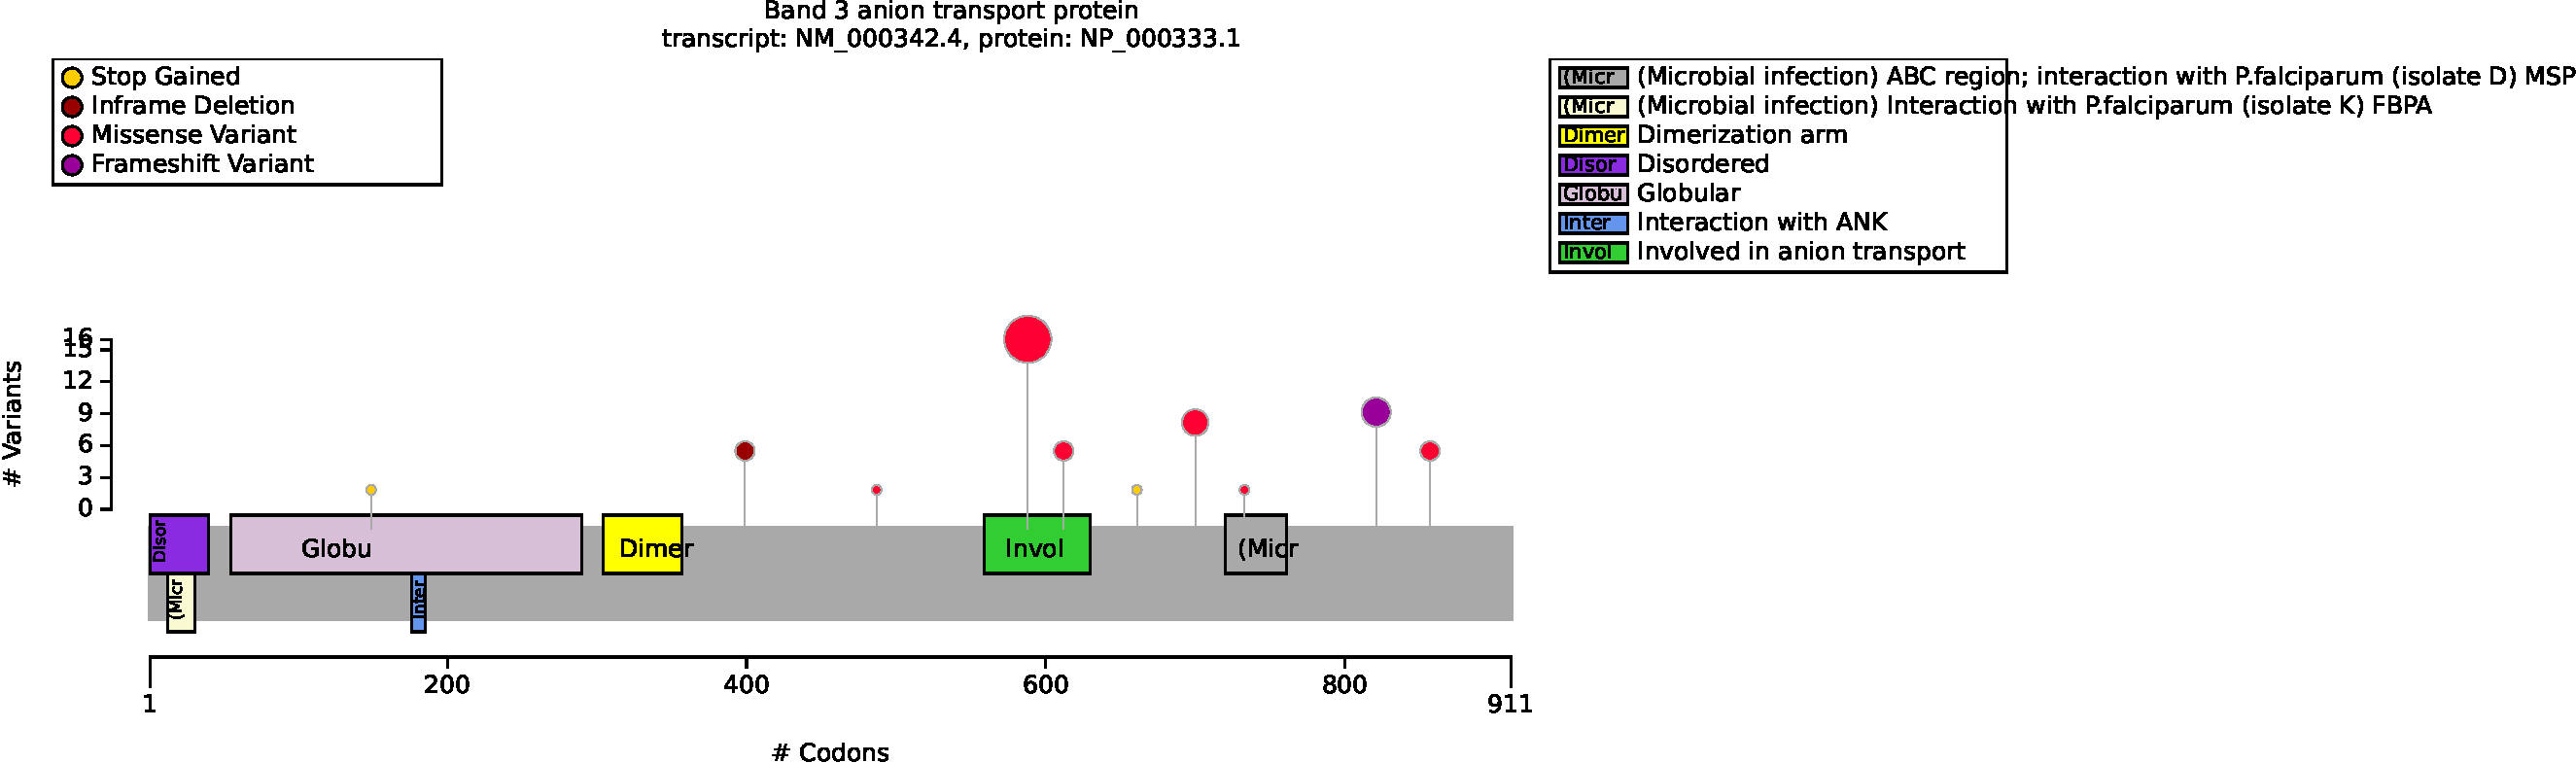
\includegraphics[width=\textwidth]{ img/SLC4A1_protein_diagram.pdf} 
\captionsetup{justification=raggedright,singlelinecheck=false}
\caption{Distribution of variants in SLC4A1}
\end{subfigure}

\vspace{2em}

\begin{subfigure}[b]{0.95\textwidth}
\centering
\resizebox{\textwidth}{!}{
\begin{tabular}{llllrr}
\toprule
Genotype (A) & Genotype (B) & total tests performed & significant results\\
\midrule
r149w & other & 14 & 0\\
\bottomrule
\end{tabular}
}
\captionsetup{justification=raggedright,singlelinecheck=false}
\caption{Fisher Exact Test performed to compare HPO annotation frequency with respect to genotypes.}
\end{subfigure}

\vspace{2em}

\caption{The cohort comprised 33 individuals (16 females, 16 males, 1 with unknown sex). A total of 49 HPO terms were used to annotate the cohort. Disease diagnoses: Distal renal tubular acidosis 1 (OMIM:179800) (18 individuals), Spherocytosis, type 4 (OMIM:612653) (7 individuals), Distal renal tubular acidosis 4 with hemolytic anemia (OMIM:611590) (7 individuals), Cryohydrocytosis (OMIM:185020) (1 individuals). No statistically significant results identified. A total of 11 unique variant alleles were found in \textit{SLC4A1} (transcript: \texttt{NM\_000342.4}, protein id: \texttt{NP\_000333.1}).}
\end{figure}
